\documentclass[12pt]{article}
\usepackage[utf8]{inputenc}
\usepackage{amsmath, amsthm, amssymb, mathrsfs}
\usepackage{tikz}
\usepackage{ctex}
\usetikzlibrary{graphs, graphs.standard,arrows.meta,positioning}
\usepackage[style=alphabetic]{biblatex}
\addbibresource{references.bib} % 创建参考文献文件

\title{$n$元集合上的传递关系数目}
\author{江李阳}
\date{\today}

\newtheorem{theorem}{Theorem}[section]
\newtheorem{lemma}[theorem]{Lemma}
\newtheorem{corollary}[theorem]{Corollary}
\theoremstyle{definition}
\newtheorem{definition}[theorem]{Definition}
\newtheorem{example}[theorem]{Example}


\begin{document}


\maketitle
\tableofcontents

%\begin{abstract}
   % This paper investigates the enumeration of transitive relations on finite sets. We present combinatorial analysis and recursive formulas for calculating the number of transitive relations on an $n$-element set. Key results include asymptotic bounds and connections to related combinatorial structures. This work extends previous research by providing new computational insights and improved lower bounds.
%\end{abstract}
\section{基本定义}
对于任意$a$,$b$,$c$$\in$$A$,(a,b)$\in$$R$并且(b,c)$\in$R,则(a,c)$\in$R,
那么定义在集合$A$上的关系$R$称为传递的.使用量词定义为:若$\forall a$$\forall b$$\forall c$ 
(((a,b)$\in$R$\bigwedge$(b,c)$\in$R)$\rightarrow $(a,c)$\in$R ),则定义在集合A上的关系称为
传递的.
\section{历史背景和研究进展}
记$T(n)$为$n$元集合上的传递关系的总数,对于一个任意的$n$元集合,一个很自然的想法就是这个集合上的传递关系数目是多少.
该问题最早由Richard P.Stanley在组合数学研究中提及,但他并未给出直接的表达式,只是记录了一些初始值.
\subsection{理论研究方向}
\subsubsection{穷举和递归算法}
对于较小的$n$,可以使用计算机穷举所有的关系并验证是否满足传递性:一个$n$元集合上总共有$2^{n^{2}}$种关系,使用位运算枚举所有的关系,
然后求解传递闭包$t(R)$,由于满足$R\subseteq t(R)$,只要满足$R=t(R)$,即可认为原关系$R$是传递的.这种方法简单直观,但是计算量随$n$成
指数级增长,只适用于非常有限的、小的$n$.
\subsubsection{与偏序关系的联系}
偏序关系(自反,反对称,传递)一定是一个传递关系,但传递关系不一定是偏序关系.通过研究偏序关系的结构分解方法可推广到一般传递关系.
\subsubsection{图论分解}
每个传递关系对应一个传递闭包,其基础图可分解为有向无环图($DAG$).将传递关系视为$DAG$的传递闭包,通过分解为强连通组件和层次结构进行计数.
\subsubsection{容斥原理和布尔矩阵}
在统计满足传递性的矩阵数时需要排除违反传递性的三元组($a,b,c$),其中存在边$a\rightarrow b$和$b \rightarrow c$但缺少$a \rightarrow c$,由于三元组间存在重叠,会重复计数,需要通过容斥原理精确计数.\\
\hspace*{2em}传递性下要求关系矩阵$M^2$$\leq$$M$,其中对$M$的乘积使用布尔运算,但这种只是判断条件,无法直接计数.
\section{现代研究成果}
\subsubsection{Comtet公式}
对于$n$元集合上的传递关系计数问题,Comtet公式通过生成函数和整数分拆给出精确的表达式:
\[
 T(n)=\sum_{k=1}^{n}\sum_{\lambda \vdash k}^{}\frac{n!}{ {\textstyle \prod_{i=1}^{k}}(m_{i}\cdot i^{m_{i}}) }\cdot 2^{ {\textstyle \sum_{i}^{}} + {\textstyle \sum_{i<j}^{} \binom{\lambda_{i}}{2}\lambda_{i}\lambda_{j}} }
\]
初始条件为$T(0)=1$,意为空集$\emptyset$上传递关系数为1.
其中$k$:传递诱导的等价类个数;$\lambda \vdash k$:遍历$k$的所有整数分拆$\lambda = (\lambda_{1},\lambda_{2},\dots ,\lambda_{m})$,满足 ${\textstyle \sum_{\lambda_{i}}^{}}=k$;
$m_i$:分拆$\lambda$中大小为$i$的块的个数;系数项:$\frac{n!}{{\textstyle \prod_{i=1}^{k}}(m_{i}\cdot i^{m_{i}})}$表示将$n$个元素分配到分拆$\lambda$指定的块结构中的方案数;指数项:$2^{\textstyle \sum_{i}^{}\binom{\lambda_{i}}{2}+\textstyle \sum_{i<j}^{}\lambda_{i}\lambda_{j} }$表示:
$\textstyle \sum_{i}^{}\binom{\lambda_{i}}{2}$表示各块内部非自反边的自由度,$\textstyle \sum_{i<j}^{}\lambda_{i}\lambda_{j}$:块间严格偏序决定的边自由度.
\\
\hspace*{2em}该公式将传递关系分解为划分+块内完全图子集+块间严格偏序,链接了整数分拆、偏序计数和等价关系计数,但计算的复杂度依然很高,需要遍历所有分拆$\lambda \vdash k$,分拆数$p(k)$增长迅速且求和形式无法化简为封闭表达式。
\subsubsection{渐进行为与上下界}
$Kleitman's\ Asymptotic\ Bounds:$Kleitman通过分析传递关系矩阵中的"1"块的结构,证明了$T(n)\leq 2^{n^2/4+o(n)}$。
核心思想为利用集合划分和链的性质来构造传递关系。特别地,他关注了关系图可以分解为若干条不相交的链的传递关系,并经过精心设计的计数和估计,给出了包含所有传递关系的范围。\\
\hspace*{2em}$2019-Sharp,Pantone,Spiro:$他们证明了$T(n)=2^{(1/4+o(1))n^2}$,核心思想为利用整数分拆来描述传递关系的结构。通过计算所有划分的权重和,证明这个和的主要贡献来自于那些块大小相对均衡的划分,最终证明最大权重对应于
块大小接近$\sqrt{n}$的划分,并且在这种划分下,可添加的自幼边数大约是$n^{2}/4$。\\
\hspace*{2em}这两个证明确定了$T(n)$的指数增长率即核心增长项为(1/4)$n^2$.
\subsubsection{精确计数与算法改进}
$Pfeiffer:$提出基于传递关系诱导的预序的树状递归结构。将问题分解为计算特定的较小的传递关系构成的更大的传递关系。这比朴素的枚举更高效。\\
$Pfreiffer\ formula:$\\
\[
T(n)=\sum_{\pi}^{}(P(k)\times \prod_{B\in \pi}^{} B(\left | B \right | ))
\]
\hspace*{2em}$\sum_{\pi}^{}$求和范围表示遍历集合$S$的所有划分$\pi$;块数$k=\left | \pi \right |$是划分$\pi$的块数(等价类的个数);
$P(k)$是$k$元集合上的偏序关系数目;$B(\left | B \right |)$贝尔数:$B(m)$是$m$元集合上的等价关系数量;乘积项$\prod_{B \in \pi}^{}B(\left | B \right |)$是对于划分$\pi$中的每个块
$B$,计算其大小$\left | B \right |$的贝尔数,并求乘积。\\
\hspace*{2em}布尔矩阵分解:传递关系看作其自反传递闭包的子集,利用布尔矩阵半环的性质,设计算法满足特的特定闭包性质的布尔矩阵数量。目前最先进的算法(基于树状分解、优化布尔矩阵计算等)已经能计算到$n$=24甚至更高。
如$T(20)$是一个有几十亿位的天文数字。
\subsubsection{随机传递关系}
研究在$n$元集合所有的$2^{n^{2}}$个二元关系上均匀随机选取一个关系时,该关系是传递关系的概率是$\frac{T(n)}{2^{n^{2}}}$。根据渐进结果$T(n)=2^{(1/4+o(1))n^2}$,这个概率约为
$2^{-(3/4+o(1))n^2}$,表明传递关系极其稀少。
\subsubsection{与图论和组合结构的关系}
通过研究传递关系对应的有向图的性质,传递关系尤其是拟序和偏序定义了集合上的闭包算子,其闭集形成一个格,研究这些格的性质及其计数有助于理解和研究传递关系计数。\\

\newpage
%\section{三元集合上的传递关系}
\section{三元集合上的传递关系}
三元集合$S=\{a,b,c\}$上的关系总数为$2^{3^2}=512$,其中传递关系总数为$T(3)$=171种,按图表示关系、图同构、等价类相关知识,所有传递关系的矩阵表示如下:\\

1.三个顶点孤立:三个顶点之间互相不存在边,只有自环存在或不存在两种情况\\
\begin{center}
$
\begin{pmatrix}
  1 & 0 & 0\\
  0 & 1 & 0\\
  0 & 0 & 1\\
\end{pmatrix}
$\\
% 等价类 1:完全无序,三个节点各自带自环
\begin{tikzpicture}[->,>={Stealth}, node distance=2cm]
  \node (a) at (0,0)   {a};
  \node (b) at (2,0)   {b};
  \node (c) at (1,1.5) {c};

  % 自环
  \draw (a) edge[loop above] (a);
  \draw (b) edge[loop above] (b);
  \draw (c) edge[loop above] (c);
  % 无其他非对角边
\end{tikzpicture}


\end{center}
成员数:$2^{3}$=8;
\\
\hspace*{2em}2.单向二元边:任意不同两个元素之间存在单向边,自环不影响传递性\\
\begin{center}
$
\begin{pmatrix}
  1 & 0 & 1\\
  0 & 0 & 0\\
  0 & 0 & 0\\
\end{pmatrix}
$\\
% 等价类 2:单向二元链 (c -> b),a 隔离
\begin{tikzpicture}[->,>={Stealth}, node distance=2cm]
  \node (a) at (0,0)   {a};
  \node (b) at (2,0)   {b};
  \node (c) at (1,1.5) {c};
  \draw (a) edge[bend right] (c);
  \draw (a) edge[loop above] (a);
\end{tikzpicture}

\end{center}
成员数:$\binom{3}{2}\cdot 2^{3}$=48;
\\
\hspace*{2em}3.倒V结构:任选一个中心元素,其余两个元素有指向中心元素的单向边,自环不影响传递性\\
\begin{center}
$
\begin{pmatrix}
  1 & 1 & 0\\
  0 & 1 & 0\\
  0 & 1 & 1\\
\end{pmatrix}
$\\
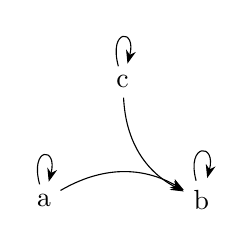
\begin{tikzpicture}[->,>={Stealth}, node distance=2cm]
  \node (a) at (0,0)   {a};
  \node (b) at (2,0)   {b};
  \node (c) at (1,1.5) {c};
  \draw (a) edge[bend left] (b);
  \draw (c) edge[bend right] (b);
  \draw (a) edge[loop above] (a);
  \draw (b) edge[loop above] (b);
  \draw (c) edge[loop above] (c);
\end{tikzpicture}\\
倒V结构:$c\rightarrow b,a \rightarrow b$
\end{center}
成员数:$\binom{3}{1}\cdot 2^{3}$=24;
\\
\hspace*{2em}4.正V结构:任选一个中心元素,中心元素指向两个剩余元素,自环不影响传递性\\
\begin{center}
$
\begin{pmatrix}
  1 & 0 & 0\\
  1 & 1 & 1\\
  0 & 0 & 1\\
\end{pmatrix}
$\\
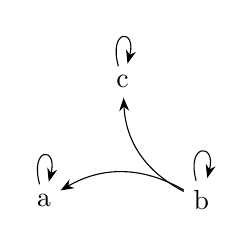
\begin{tikzpicture}[->,>={Stealth}, node distance=2cm]
  \node (a) at (0,0)   {a};
  \node (b) at (2,0)   {b};
  \node (c) at (1,1.5) {c};
  \draw (b) edge[bend right] (a);
  \draw (b) edge[bend left] (c);
  \draw (a) edge[loop above] (a);
  \draw (b) edge[loop above] (b);
  \draw (c) edge[loop above] (c);
\end{tikzpicture}\\
正V结构:$b\rightarrow c,b \rightarrow a$
\end{center}
成员数:$\binom{3}{1}\cdot 2^{3}$=24;
\\
\hspace*{2em}5.二元循环:任选一个孤立元素,是否存在自环不影响传递性,剩余两个元素之间形成双向有向边和自环\\
\begin{center}
$
\begin{pmatrix}
  1 & 0 & 0\\
  0 & 1 & 1\\
  0 & 1 & 1\\
\end{pmatrix}
$\\
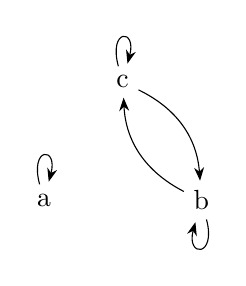
\begin{tikzpicture}[->,>={Stealth}, node distance=2cm]
  \node (a) at (0,0)   {a};
  \node (b) at (2,0)   {b};
  \node (c) at (1,1.5) {c};
  \draw (b) edge[bend left] (c);
  \draw (c) edge[bend left] (b);
  \draw (a) edge[loop above] (a);
  \draw (b) edge[loop below] (b);
  \draw (c) edge[loop above] (c);
\end{tikzpicture}\\
孤立元素$a$,二元循环$c\rightleftarrows  b,\circlearrowleft b \circlearrowleft c$
\end{center}
成员数:$\binom{3}{1}\cdot 2^{1}$=6;
\\
\hspace*{2em}6.严格三元三边:存在有向边$i\rightarrow j$,$j \rightarrow k$,及传递性产生的边$ i \rightarrow k$,自环不影响传递性\\
\begin{center}
$
\begin{pmatrix}
  0 & 1 & 1\\
  0 & 0 & 1\\
  0 & 0 & 0\\
\end{pmatrix}
$\\
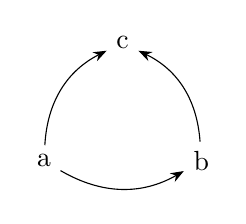
\begin{tikzpicture}[->,>={Stealth}, node distance=2cm]
  \node (a) at (0,0)   {a};
  \node (b) at (2,0)   {b};
  \node (c) at (1,1.5) {c};
  \draw (a) edge[bend right] (b);
  \draw (a) edge[bend left] (c);
  \draw (b) edge[bend right] (c);
\end{tikzpicture}\\
三边:$a\rightarrow b,b \rightarrow c$,$c \rightarrow a$
\end{center}
成员数:$\binom{3}{1}\cdot \binom{2}{1}\cdot 2^{3}$=48;
\\
\hspace*{2em}8.二元循环且指向"孤立点":任选两个元素形成二元循环且都向剩余元素形成指向边,剩余一个元素自环不影响传递性\\
\begin{center}
$
\begin{pmatrix}
  0 & 0 & 0\\
  1 & 1 & 1\\
  1 & 1 & 1\\
\end{pmatrix}
$\\
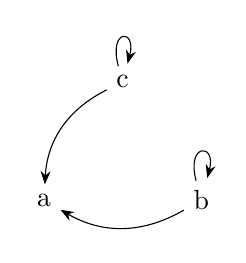
\begin{tikzpicture}[->,>={Stealth}, node distance=2cm]
  \node (a) at (0,0)   {a};
  \node (b) at (2,0)   {b};
  \node (c) at (1,1.5) {c};
  \draw (b) edge[bend left] (a);
  \draw (c) edge[bend right] (a);
  \draw (b) edge[loop above] (b);
  \draw (c) edge[loop above] (c);
\end{tikzpicture}\\
二元循环:$c\rightleftarrows b,b \rightarrow b,c \rightarrow c$,与剩余元素之间的指向边:$b \rightarrow a,c \rightarrow a$
\end{center}
成员数:$\binom{3}{1}\cdot 2^{1}$=6;
\\\hspace*{2em}9.全连通:三个元素之间都存在双向有向边\\
\begin{center}
$
\begin{pmatrix}
  1 & 1 & 1\\
  1 & 1 & 1\\
  1 & 1 & 1\\
\end{pmatrix}
$\\
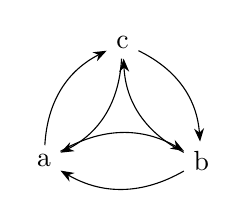
\begin{tikzpicture}[->,>={Stealth}, node distance=2cm]
  \node (a) at (0,0)   {a};
  \node (b) at (2,0)   {b};
  \node (c) at (1,1.5) {c};
  %\draw (a) edge (b);
  %\draw (a) edge (c);
  %\draw (b) edge (a);
  \draw (a) edge[bend left](b);
  \draw (b) edge[bend left](a); 
   \draw (a) edge[bend left](c);
  \draw (c) edge[bend left](a); 
   \draw (b) edge[bend left](c);
  \draw (c) edge[bend left](b); 
 % \draw (b) edge (c);
  %\draw (c) edge (a);
  %\draw (c) edge (b);
\end{tikzpicture}\\
三个元素之间都存在双向有向边:$a \rightleftarrows b ,b \rightleftarrows c,b \rightleftarrows c$
\end{center}
成员数:$2^{0}$=1;
\\
\hspace*{2em}总计3元集合上的传递关系数目:$T(3)=8+48+24+24+6+48+6+1=171$

\end{document}